\section{Багатошаровий перцептрон}

Одним із найкращих за якістю алгоритмів машинного навчання є
багатошаровий перцептрон. У багатошаровому перцептроні існує
можливість використання більше ніж одного лінійного шару (рис. \ref{fig:mlp}).
Розглянемо на прикладі звичайну тришарову нейронну мережу перцептрона:
перший шар називається вхідним, середній шар --- прихованим,
що і є головною відмінністю від перцептрона Розенблата, а останній шар ---
вихідним.

Спочатку йде подача інформації до вхідного шару і на виході отримуємо
результат моделі. У цій мережі, звісно, можна збільшувати кількість
прихованих шарів нейронів, що в результаті дасть якісніший результат,
але при цьому сильно зросте використання обчислювальних ресурсів. Тому
дуже важливо правильно налаштовувати так звані гіперпараметри,
від яких залежить швидкість та якість обробки.

\begin{figure}[H]
  \centering
  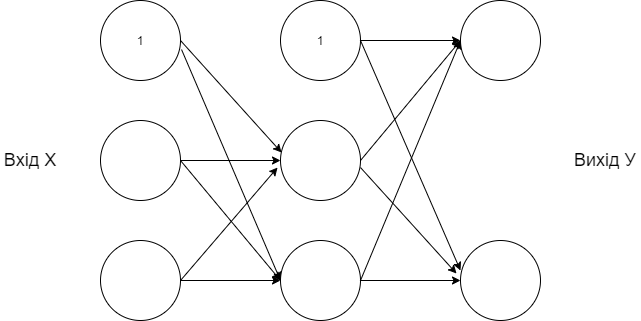
\includegraphics[width=0.7\textwidth]{images/image16}
  \caption{Приклад багатошарового перцептрона}
  \label{fig:mlp}
\end{figure}

Одними з ключових характеристик багатошарового перцептрона є
використання нелінійної функції активації, як правило, сигмоїдної. Також
у ньому, як уже було сказано, число шарів, які навчаються, більше одного. У
загальних випадках використовують не більше трьох.

Сигнали, що одержує модель, можуть бути інтерпретовані у десяткових
числах. Після цього бажано провести нормалізацію даних значень. Це
потрібно робити, оскільки функція активації є сигмоїдальною і приймає
значення від 0 до 1.

Навчання багатошарового перцептрона проводиться до стабілізації
коефіцієнтів під час навчання або зупиняється, не дійшовши до кінця навчання,
щоб уникнути перенавчання.
